\section{Kalman Filter} \label{sec:KalmanFilter}
This section describes the theory behind and implementation of a Kalman filter used for sensor fusion and tracking of a person in this project.\\

The sensors described in chapter \ref{ch:equipment} measure data with some noise, giving readings that are not completely reliable. Additionally, as more sensors are used to track the same person, these must be fused, using an algorithm, in order to ensure the best estimate of the position of people. Both the fusion of sensors and reduction of noise in measurements can be achieved by implementing a Kalman filter for tracking people.\\

The Kalman filter supplies a recurring method for estimating the state of a dynamic system when the system contains noise. The Kalman filter maintains estimates of the state vector ($\hat{x}$) and the error covariance matrix ($P$) of the system. This assumes that the system has a Gaussian probability density function (PDF) as an output with the mean $\hat{x}$ and covariance $P$. In the context of tracking people this means that the estimated position, calculated using the Kalman filter, is a distribution of likely positions rather than a particular position.\\

%Insert some picture if it makes sense

As mentioned previously, the Kalman filter is a recurring function running in two steps, prediction and update. The first step, prediction, takes the known parameters of the system to estimate the current state of the system $\hat{x}(k+1|k)$ along with the covariance propagation $P(k+1|k)$. With the predicted state of the system calculated, the sensor measurements can be compared to the prediction to compute the updated state of the system. This is done in the update step where the Kalman gain ($K$) is computed based on the estimated covariance and the sensor noise. The Kalman gain is then used to compute the updated state of the system by combining the predicted state with the sensor measurements to determine the new Gaussian PDF for the time step ($k+1$). The Kalman gain is used to determine the weighted average of the prediction and the measurements, dependant on the uncertainty of each value.\cite{choset2005principles}

\subsubsection{Prediction step}
As described above, the prediction step predicts the state and covariance of the system. This is done in the following two functions:

\begin{equation}
\hat{x}(k+1|k) = F(k)\hat{x}(k|k)+u(k)
\end{equation}
which is the prediction of the mean of the position and,
\begin{equation}
P(k+1|k) = F(k)P(k|k)F(k)^T+Q(k)
\end{equation}
which is the prediction of the covariance of the position.

Where:
\begin{itemize}
    \item $\hat{x}$: Estimation vector
    \item $k$: Kalman gain
    \item $F$: The state transition matrix
    \item $u$: Control vector adding any known changes to the system 
    \item $P$: Prediction matrix
    \item $Q$: Overall process noise in a covariance matrix.
\end{itemize}
\vspace*{5mm}

%where \textit{F} is the state transition matrix, depicting the base change of \textit{x} and \textit{P}, and \textit{u} is the control vector adding any known changes to the system (such as a change in velocity of the observer).

%where \textit{Q} is an overall process noise in a covariance matrix.

\subsubsection{Update step}
The update step combines the prediction with the sensor measurements as described previously. This is calculated in the following two functions:
\begin{equation}
\hat{x}(k+1|k+1) = \hat{x}(k+1|k) + Ky
\label{eq:kalmanupdate1}
\end{equation}
which is the updated mean of the position and,
\begin{equation}
P(k+1|k+1) = (I - (K * H(k+1)) P(k+1|k)
\label{eq:kalmanupdate2}
\end{equation}
which is the update of the covariance of the position.

Where:
\begin{itemize}
    \item $y$: Measurement residual
    \item $I$: Identity matrix 
    \item $H$: Vector mapping matrix
\end{itemize}
\vspace*{5mm}

%where \textit{K} is the Kalman gain and \textit{y} is the measurement residual, the difference between measured and expected values.

In both equation \ref{eq:kalmanupdate1} and \ref{eq:kalmanupdate2}, the $K$ is calculated by $K=PH(k+1)^TS^{-1}$, where $S$ is a residual covariance matrix that is increased by measurement noise. Additionally, the $y$ is calculated $y = Z(k+1)^T - H(k+1)x$, where $Z$ is measurements from the sensors.\\

With the general description of the Kalman filter concluded, the implementation of the filter for this project can be explained.

\subsection{Implementation of the Kalman Filter}

The Kalman filter is used for fusing the data from the leg detection and face detection in this project and publishing the data to the implemented velocity controller.
The Kalman filter is implemented through the use of a python library called pykalman\cite{pykalman}. This is the reason for the ROS node Kalman filter being written in python rather than in C++ as the other nodes.
The pykalman needs six initiations matrices, transition ($F$), observation ($H$), transition covariance ($Q$), initial observation covariance ($R0$), initial estimation ($X0$) and initial prediction ($P0$), this is called every time a new Kalman filter object is created. This Kalman filter is implemented in such a way that it works best on updating it with a approximately same time step, meaning updating the filter at frequency, with or without new measurements. This requires The ROS node to run at a frequency that is able to handle data, published at different frequencies, this is done be updating at higher frequency than is published on any of the topics. To ensure that if data arrives at the same time a boolean is used to only allow one update per time step. If the Kalman filter updates without any new measurements from the two topics, it will update on the previous estimate of the person and prediction made.\\

\begin{figure}[H]
    \centering
    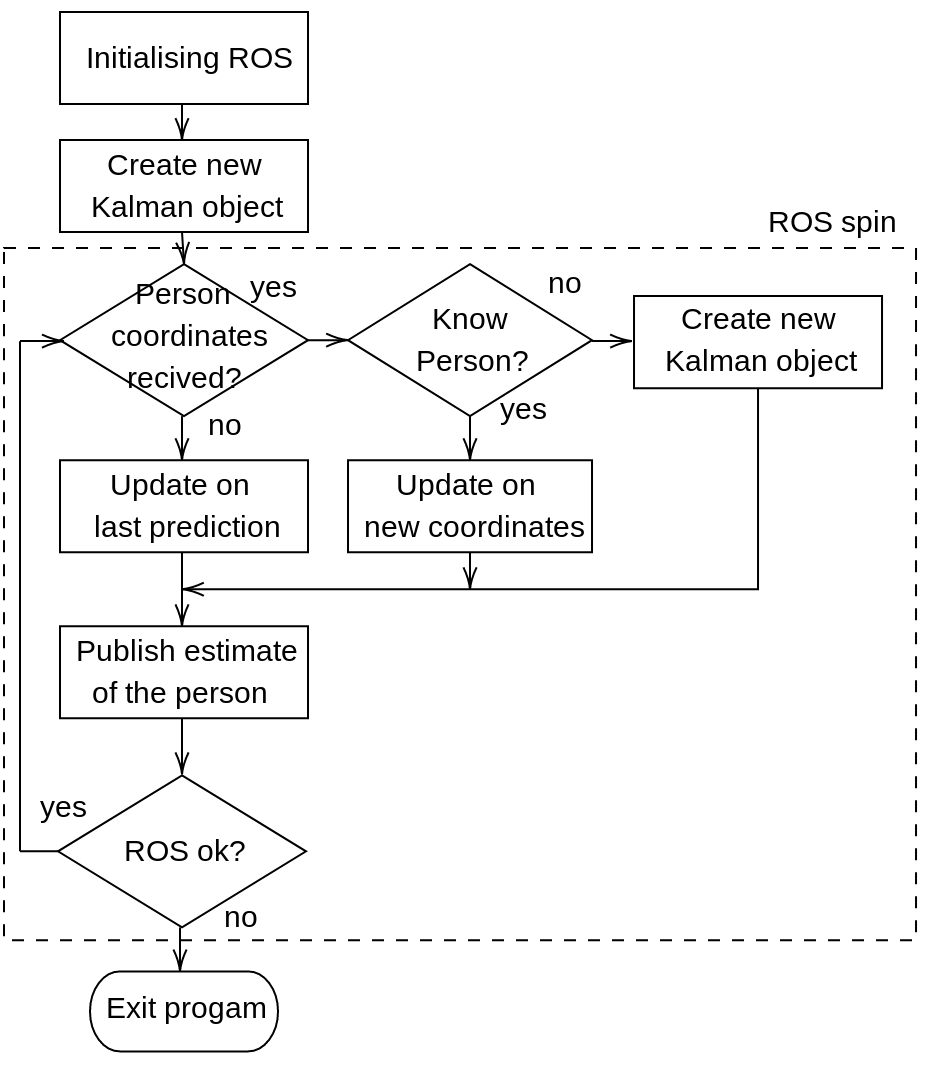
\includegraphics[width=0.65\textwidth]{figures/flow_pykalman.png}
    \caption{Flow chart of implementation of node running the Kalman filter}
    \label{fig:flow_pykalman}
\end{figure}

When a person is first detected on the leg detection topic, it stores the persons data. A helper class is created to hold the values of the persons evaluated, i.e the x,y coordinates and a name. The name of the person that is received from the leg detector node, to compare if it is a new person or if it is the same as previous detected. If the person is the same it will update the Kalman filter with the $k-1$ estimate of position, the $k-1$ prediction, the observation and the observation covariance. The new updated estimate of the x and y position from the Kalman filter is published to the speed controller. If it is a new person that has been discovered a new initialisation of the Kalman filter is created, as previous mentioned with initial matrices.\\
If a message is received on the face detector topic, the Kalman filter will only update the Kalman filter with the received data due to the way of implementation of the face detector. The face detector does not check if the image that it analyses is the same person. Every time this node filters and publishes it is done through the same method in the class that is named Kalman in this project. This method is named filter and pub, it requires two arguments to be passed to the observation and the covariance observation. These arguments are used to update the Kalman filter, if there is no new input from the sensors, the keyword none is passed in as the observation and observation covariance, to make the Kalman filter only update in the previous estimate and prediction. This method keeps track of the time and ensures that the update frequency and the new estimate is published correctly, by the use of rospy.sleep function, that is set to the specified rate, and rospy.spin.